\begin{frame}{Types of Outcome Variable}
    \begin{itemize}
        \item So far, all of our outcome variables have been numeric.
        \item Values of $\hat{y}$ are continuous numeric.
        \item What happens when we have categorical outcomes?
        \item Enter \textbf{logistic regression}.
    \end{itemize}
\end{frame}

\begin{frame}{Generalized Linear Models}
    (Multiple) linear regression and logistic regression are both a type of \textbf{generalized linear model (GLM)}.
    \begin{itemize}
        \item Logistic regression will allow us to model binary response variables.
        \item That is, we will be able to model categorical variables with two levels.
    \end{itemize}
\end{frame}

\begin{frame}{Generalized Linear Models}
    We can think of GLMs as a two-stage approach:
    \begin{enumerate}
        \item Model the response variable using some probability distribution.
        \item Model the distribution's parameter(s) using a collection of predictors (as in multiple regression).
    \end{enumerate}
\end{frame}

\begin{frame}{Generalized Linear Models}
    We've already been doing this! 
    
    \vspace{12pt}For a continuous outcome,
    \begin{enumerate}
        \item The response variable is assumed to follow a normal distribution.
        \item The mean of this normal distribution is $\beta_0 + \beta_1x_1 + \dots + \beta_kx_k$.
    \end{enumerate}
\end{frame}

\begin{frame}{Example: Resume Data}
    Consider data from a study to examine the effect of race and sex on job application callback rates. 
    \begin{itemize}
        \item Fake resumes were sent to job ads in Boston and Chicago.
        \item Researchers wanted to see which would elicit callbacks.
        \item Experience and education were randomly generated.
        \item Finally, names were randomly generated and added to the resumes.
        \begin{itemize}
            \item Names were generated such that hiring managers would be likely to assume both race and gender.
        \end{itemize}
    \end{itemize}
\end{frame}

\begin{frame}{Example: Resume Data}
    The response variable of interest is
    \[
        \texttt{callback} = 
        \begin{cases}
        1 \quad \text{if} \quad \text{received callback} \\
        0 \quad \text{otherwise}
        \end{cases}
    \]
\end{frame}

\begin{frame}{Example: Resume Data}
    The variables in this dataset are
    \begin{table}
    \centering
    \begin{tabular}{ll}
        \texttt{callback} & yes or no  \\
        \texttt{job\_city} & Boston or Chicago \\
        \texttt{college\_degree} & yes or no \\
        \texttt{years\_experience} & Numeric, number of years experience\\
        \texttt{honors} & Resume lists some type of honors, yes or no \\
        \texttt{military} & yes or no \\
        \texttt{email\_address} & Listed, yes or no \\
        \texttt{race} & Black or white (implied by name) \\
        \texttt{sex} & implied by name
    \end{tabular}
    \end{table}
\end{frame}

\begin{frame}{Example}
    Race and sex are protected classes in the US, meaning that employers are not legally allowed to make hiring decisions based on these factors.
    
    \vspace{12pt} This study...
    \begin{itemize}
        \item has random assignment.
        \item is a true experiment.
    \end{itemize}
    
    \vspace{12pt}Therefore we may infer causation between (statistically significant) variables and the callback rate.
\end{frame}

\begin{frame}{Modeling the Probability of an Event}
    With logistic regression,
    \begin{itemize}
        \item The outcome $Y_i$ takes values 1 or 0 with some probability.
        \begin{itemize}
            \item $P(Y_i = 1) = p_i$
            \item $P(Y_i = 0) = 1-p_i$
        \end{itemize}
        \item The subscript $i$ refers to the $i$th observation (in this case the $i$th resume).
        \item We will model the probability $p$, which takes values $p_1, \dots, p_n$.
    \end{itemize}
\end{frame}

\begin{frame}{Logistic Regression}
    We want to relate the probability of a callback for each resume, $p$, to the predictors $x_1, \dots, x_k$. 
    
    \vspace{12pt}This will look a lot like multiple regression!
    \[
    \text{transformation}(p) = \beta_0 + \beta_1x_1 + \dots + \beta_kx_k + \epsilon
    \]
\end{frame}

\begin{frame}{Transforming $p$}
    Why do we transform $p$?
    
    \vspace{12pt}\begin{itemize}
        \item We want the range of possibilities for the outcome to match the range of $p$
        \begin{itemize}
            \item $p = P(Y=1)$ is between 0 and 1!
        \end{itemize}
        \item Without a transformation, $\beta_0 + \beta_1x_1 + \dots + \beta_kx_k$ could take values outside of 0 to 1.
    \end{itemize}
\end{frame}

\begin{frame}{Transforming $p$}
    A common transformation for $p$ is the \textbf{logit transformation}:
    \[
        \text{logit}(p) = \log\left(\frac{p}{1-p}\right)
    \]
\end{frame}

\begin{frame}{The Logistic Model}
    Then the model looks like
    \vspace{12pt}\Large{\[
        \log\left(\frac{p}{1-p}\right) = \beta_0 + \beta_1x_1 + \dots + \beta_kx_k + \epsilon
    \]}
\end{frame}

\begin{frame}{Example: Transforming the Resume Data}
    \begin{center}
        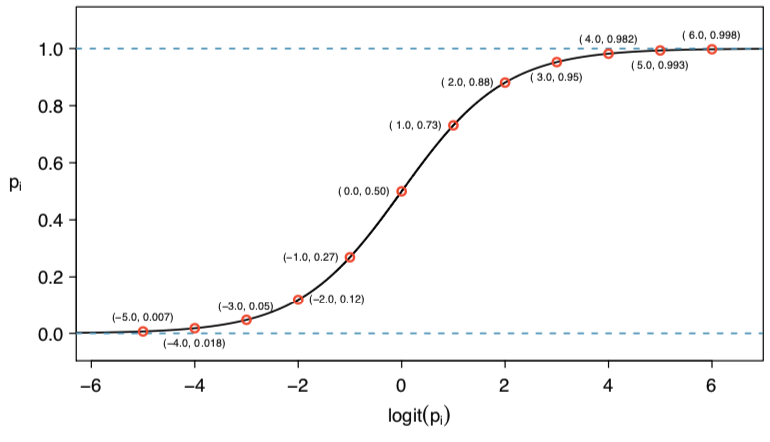
\includegraphics[width=4.5in]{images/logit.png}
    \end{center}
\end{frame}

\begin{frame}{Example: Fitting the Model}
    We start with the model that includes only \texttt{honors}.
    \[
        \log\left(\frac{p}{1-p}\right) = -2.4998 + 0.8668\times\texttt{honors}
    \]
    For a resume with no honors listed, what is the probability of a callback?
\end{frame}

\begin{frame}{A Note}
    As with multiple regression, we'll fit all of these models using a computer (the computer will do the logit transformation for you, too!), but we do need to know how to interpret the results.
\end{frame}

\begin{frame}{Converting Back to probabilities}
    To make probability predictions using a logistic regression, use
    
    \vspace{12pt}\Large{
    \[
        p = \frac{e^{\beta_0 + \beta_1x_1 + \dots + \beta_kx_k}}{1 \; + \; e^{\beta_0 + \beta_1x_1 + \dots + \beta_kx_k}}
    \]
    }
\end{frame}

\begin{frame}{Example: Resume Data}
    The summary for the full model is
    \begin{table}[h]
        \centering
        \begin{tabular}{l rrrr}
            \hline
                    & Estimate & Std. Error & z value & Pr$(>|$z$|)$ \\
            \hline
(Intercept)         & -2.6632 & 0.1820 & -14.64 & $<$0.0001 \\
job\_city:Chicago   & -0.4403 & 0.1142 & -3.85 & 0.0001 \\
college\_degree     & -0.0666 & 0.1211 & -0.55 & 0.5821 \\
years\_experience   & 0.0200 & 0.0102 & 1.96 & 0.0503 \\
honors              & 0.7694 & 0.1858 & 4.14 & $<$0.0001 \\
military            & -0.3422 & 0.2157 & -1.59 & 0.1127 \\
email\_address      & 0.2183 & 0.1133 & 1.93 & 0.0541 \\
race:white          & 0.4424 & 0.1080 & 4.10 & $<$0.0001 \\
sex:male            & -0.1818 & 0.1376 & -1.32 & 0.1863 \\
            \hline
        \end{tabular}
    \end{table}
\end{frame}

\begin{frame}{Variable Selection for Logistic Regression}
    \begin{itemize}
        \item The approach is similar to using $R^2_{adj}$ in multiple regression.
        \item Use a statistic called \textbf{Akaike information criterion (AIC)}.
        \begin{itemize}
            \item This is similar to $R^2_{adj}$ in that it balances model fit and number of parameters.
        \end{itemize}
        \item We will prefer models with a \textit{lower} AIC value.
    \end{itemize}
\end{frame}

\begin{frame}{Variable Selection for Logistic Regression}
    Running all possible seven-variable models for the resume data, the model with the lowest AIC has \texttt{college\_degree} removed.
    \begin{table}[h]
        \centering
        \begin{tabular}{l rrrr}
            \hline
                    & Estimate & Std. Error & z value & Pr$(>|$z$|)$ \\
            \hline
(Intercept)         & -2.7162 & 0.1551 & -17.61 & $<$0.0001 \\
job\_city:Chicago   & -0.4364 & 0.1141 & -3.83 & 0.0001 \\
years\_experience   & 0.0206 & 0.0102 & 2.02 & 0.0430 \\
honors              & 0.7634 & 0.1852 & 4.12 & $<$0.0001 \\
military            & -0.3443 & 0.2157 & -1.60 & 0.1105 \\
email\_address      & 0.2221 & 0.1130 & 1.97 & 0.0494 \\
race:white          & 0.4429 & 0.1080 & 4.10 & $<$0.0001 \\
sex:male            & -0.1959 & 0.1352 & -1.45 & 0.1473 \\
            \hline
        \end{tabular}
    \end{table}
    Notice that the coefficients barely changed!
\end{frame}

\begin{frame}{The Logistic Regression Model}
    \begin{itemize}
        \item Sex is not statistically significant.
        \item However, race is associated with a near-zero p-value.
        \begin{itemize}
            \item The coefficient corresponds to \texttt{white}.
            \item To interpret this coefficient, we would say that the \textit{probability of callback} is higher for \texttt{white}.
            \item These data provide very strong evidence for racial bias in job application callbacks.
        \end{itemize}
    \end{itemize}
\end{frame}

\begin{frame}{Example}
        \begin{table}[h]
        \centering
        \begin{tabular}{l rrrr}
            \hline
                    & Estimate & Std. Error & z value & Pr$(>|$z$|)$ \\
            \hline
(Intercept)         & -2.7162 & 0.1551 & -17.61 & $<$0.0001 \\
job\_city:Chicago   & -0.4364 & 0.1141 & -3.83 & 0.0001 \\
years\_experience   & 0.0206 & 0.0102 & 2.02 & 0.0430 \\
honors              & 0.7634 & 0.1852 & 4.12 & $<$0.0001 \\
military            & -0.3443 & 0.2157 & -1.60 & 0.1105 \\
email\_address      & 0.2221 & 0.1130 & 1.97 & 0.0494 \\
race:white          & 0.4429 & 0.1080 & 4.10 & $<$0.0001 \\
sex:male            & -0.1959 & 0.1352 & -1.45 & 0.1473 \\
            \hline
        \end{tabular}
    \end{table}
    Write the logistic regression model for these data.
\end{frame}

\begin{frame}{Example}
        \begin{table}[h]
        \centering
        \begin{tabular}{l rrrr}
            \hline
                    & Estimate & Std. Error & z value & Pr$(>|$z$|)$ \\
            \hline
(Intercept)         & -2.7162 & 0.1551 & -17.61 & $<$0.0001 \\
job\_city:Chicago   & -0.4364 & 0.1141 & -3.83 & 0.0001 \\
years\_experience   & 0.0206 & 0.0102 & 2.02 & 0.0430 \\
honors              & 0.7634 & 0.1852 & 4.12 & $<$0.0001 \\
military            & -0.3443 & 0.2157 & -1.60 & 0.1105 \\
email\_address      & 0.2221 & 0.1130 & 1.97 & 0.0494 \\
race:white          & 0.4429 & 0.1080 & 4.10 & $<$0.0001 \\
sex:male            & -0.1959 & 0.1352 & -1.45 & 0.1473 \\
            \hline
        \end{tabular}
    \end{table}
    Write the logistic regression model for these data.
\end{frame}

\begin{frame}{Example}
    Use the logistic regression model to estimate the probability of receiving a callback for a job in Chicago where the candidate lists 14 years experience, no honors, no military experience, includes an email address, and has a first name that implies they are a White male.
    
    \vspace{12pt}...then calculate the probability of receiving a callback for a candidate who is the same on all characteristics but race.
    
    \vspace{18pt}On average, how many jobs does each candidate need to apply to in order to receive a callback?
\end{frame}

\begin{frame}{Resume Data}
    \begin{itemize}
        \item This is a simplified version of the actual data used in the 2003 article.
        \begin{itemize}
            \item The full data produced the same basic conclusions.
        \end{itemize}
        \item Because regression is about trends or averages, it is impossible (using this data) to point fingers at any particular employer or hiring managers.
        \item All we can say for sure is that the data shows a clear racial bias in job callbacks. 
    \end{itemize}
\end{frame}

\begin{frame}{Logistic Regression Diagnostics}
    There are two key conditions for the logistic regression model:
    \begin{enumerate}
        \item Each outcome $y_i$ is independent of the other outcomes.
        \item Each predictor $x_i$ is linearly related to logit$(p_i)$ if all other predictors are held constant.
    \end{enumerate}
    
    \vspace{12pt}Note: the linear regression assumptions of constant variance and normally distributed residuals come from the normal model.
    
    \vspace{12pt}In a logistic regression, we assume a binomial model. 
\end{frame}

\begin{frame}{Diagnostics for the Callback Rate Model: Independence}
    \textit{Independence} is satisfied because the resume characteristics were randomly assigned.
\end{frame}

\begin{frame}{Diagnostics for the Callback Rate Model: Linearity}
    \begin{itemize}
        \item It is difficult to check linearity without a fairly large dataset.
        \item Fortunately, the resume data has 4870 entries.
    \end{itemize}
\end{frame}

\begin{frame}{Diagnostics for the Callback Rate Model}
    We want to assess the quality of the model. 
    
    \vspace{12pt}Ex: if we look at resumes that we modeled as having a 10\% chance of getting a callback, do we find about 10\% of them actually receive a callback?
\end{frame}

\begin{frame}{Diagnostics for the Callback Rate Model}
    \begin{center}
        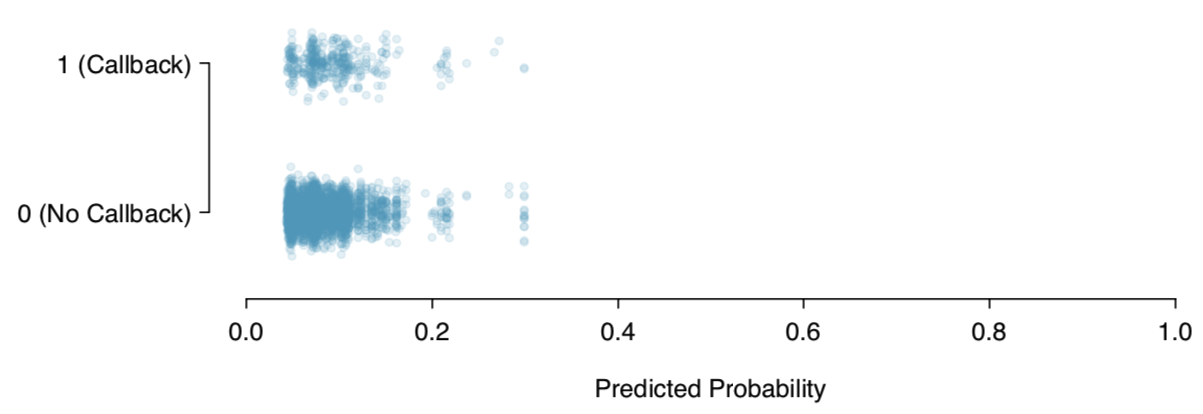
\includegraphics[width=4.5in]{images/predreallog.png}
    \end{center}
    We will start to think about this using a plot.
\end{frame}

\begin{frame}{Diagnostics for the Callback Rate Model}
    We will add to this plot as follows:
    \begin{enumerate}
        \item Bucket the data into groups based on predicted probabilities.
        \item Compute the average predicted probability for each group.
        \item Compute the observed probability for each group along with 95\% confidence intervals.
        \item Plot the observed probabilities (with the confidence intervals) against the average predicted probabilities for each group.
    \end{enumerate}
\end{frame}

\begin{frame}{Diagnostics for the Callback Rate Model}
    \begin{center}
        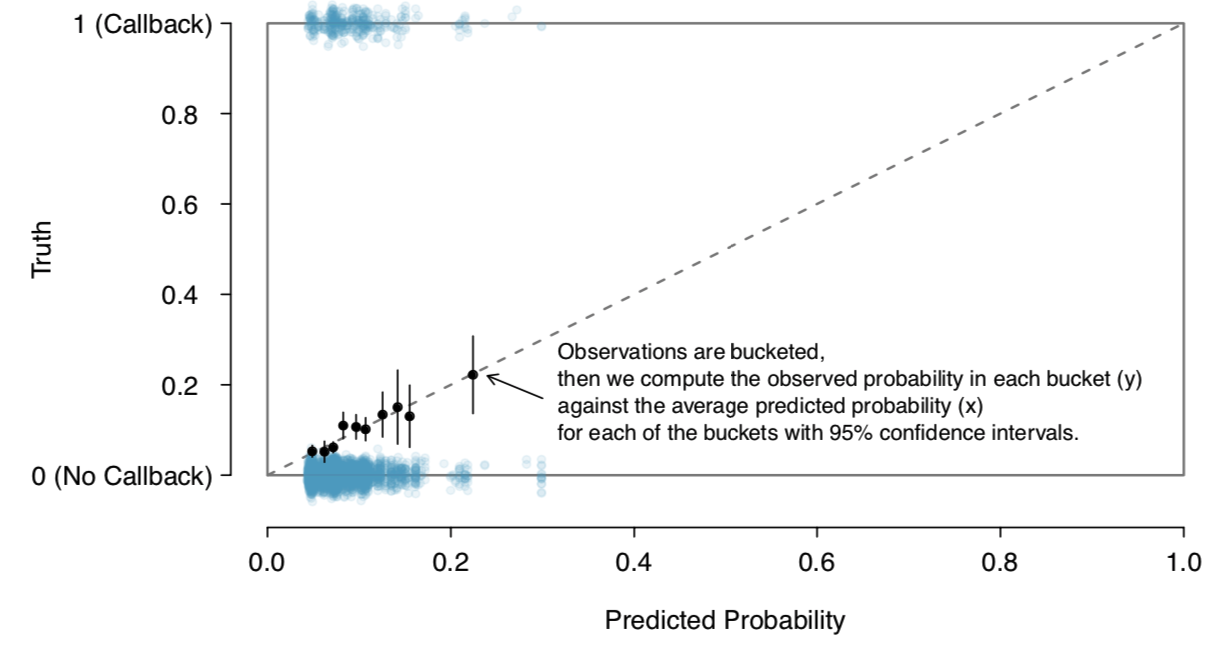
\includegraphics[width=4.5in]{images/logdiag.png}
    \end{center}
\end{frame}

\begin{frame}{Groups of Different Sizes}
    Section 9.5 closes with an interesting probability problem.
    \begin{itemize}
        \item In the resume data, we found that individuals with names perceived to be from a Black person would have to send $\approx50\%$ more resumes in order to receive a callback.
        \item We want to consider other dimensions to this.
    \end{itemize}
\end{frame}

\begin{frame}{Example}
    Consider a hypothetical company made up of 20\% women and 80\% men.
    \begin{itemize}
        \item Suppose the company has $20,000$ employees.
        \item Whenever someone goes up for promotion, 5 of their colleagues are randomly chosen to provide feedback on their work.
        \item Now suppose that in this company, 10\% of the people are prejudiced against the other sex.
    \end{itemize}
    \vspace{12pt}How often will people experience sex-based discrimination?
\end{frame}

\begin{frame}{Groups of Different Sizes}
    This is a very simplified example, but we've used probability to highlight something:
    \begin{itemize}
        \item Even when both groups are equally discriminatory, the smaller group will experience more discrimination.
        \item Increasing the imbalance in population size increases this discrepancy. 
    \end{itemize}
    \vspace{12pt}There is a lot of nuance being left out here, but nonetheless this is an important probability property to be aware of.
\end{frame}

\begin{frame}{Example: 9.17 Possum classification, Part II. }
    A logistic regression model was proposed for classifying common brushtail possums into their two regions. The outcome variable took value 1 if the possum was from Victoria and 0 otherwise.
    \begin{center}
        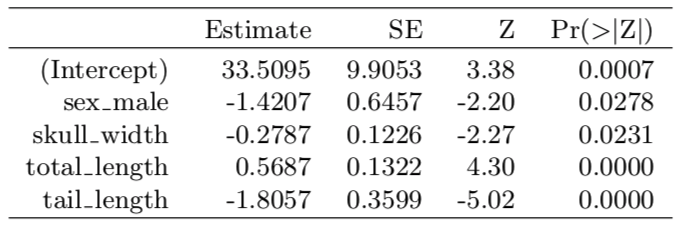
\includegraphics[width=3.5in]{images/possumprob.png}
    \end{center}
    \begin{itemize}
        \item Write out the form of the model. Also identify which of the variables are positively associated when controlling for other variables. 
    \end{itemize}
\end{frame}

\begin{frame}{Example: 9.17 Possum classification, Part II. }
    \begin{center}
        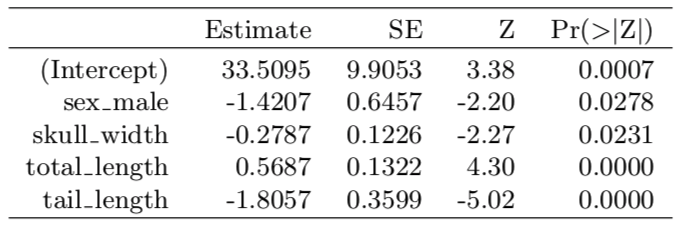
\includegraphics[width=3.5in]{images/possumprob.png}
    \end{center}
    \vspace{-18pt}\begin{itemize}
        \item Suppose we see a brushtail possum at a zoo in the US, and a sign says the possum had been captured in the wild in Australia, but it doesn’t say which part of Australia. However, the sign does indicate that the possum is male, its skull is about 63 mm wide, its tail is 37 cm long, and its total length is 83 cm. What is the model’s computed probability that this possum is from Victoria? How confident are you in the model’s accuracy of this probability calculation?
    \end{itemize}
\end{frame}
